\section{Estampa de tiempo}

Antes de entrar a la explicación sobre los sistemas de detección de intrusos, se van a definir las etapas que surgen antes de que suceda un incidente de seguridad en donde en el proceso de una de esas etapas se encuentra el funcionamiento de los sistemas de detección de intrusos.\\

Basados en lo que nos hace mención en el NIST, para llegar a una etapa en donde ocurre un incidente de seguridad se tuvo que haber pasado por otras tres etapas anteriores. La estampa de tiempo consta de tres etapas: Ataque, Intrusión e Incidente. Si en dicha estampa de tiempo se logra traspasar la etapa de un incidente, ya es considerado como un evento de seguridad.\\ 

\begin{figure}
	\centering
	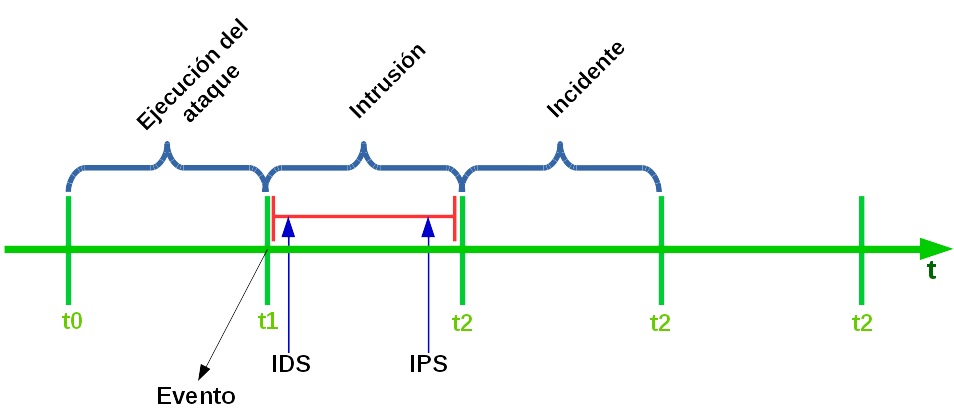
\includegraphics[scale=.4]{images/time_stamp}
	\caption{Estampa de tiempo describiendo las etapas de un evento de seguridad.}
	\label{fig:time_stamp}
\end{figure}

En la Figura \ref{fig:time_stamp} se pueden ver las etapas con respecto al tiempo para la generación de un evento de seguridad. Las etapas se pueden definir como:\\
\begin{enumerate}
	\item \textbf{Ataque:} Explotación de una vulnerabilidad.
	\item \textbf{Evento:} Lo ocasionado por un ataque identificado, y en la mayoría con resultado, exitoso.
	\item \textbf{Intrusión:} Acceso a redes no autorizadas, cuando se logra traspasar la primera linea de controles de seguridad.
	\item \textbf{Incidente:} Lo posterior a un resultado no autorizado. Violación or am	enaza inminente de violación de las políticas de seguridad.
\end{enumerate}


Una vez conocido las etapas por las que se debe de pasar para considerar que se ha generado un incidente de seguridad, se puede proceder a ver la taxonomía de un incidente de seguridad. Es importante el conocimiento de en dónde se ubica cada etapa debido a que dependiendo de la información que se tenga y la etapa en la que se encuentre, el manejo de los términos cambia y con ello los controles de seguridad que deben entrar en acción. En la Figura \ref{fig:tax_seg} se muestra la taxonomía de los incidentes de seguridad, como se puede observar, en cada una de las etapas existe un bloque de información que se debe conocer para poder hacer uso del término. Si bien, cada etapa es acumulativa lo que implica que sea complementada con la información obtenida de la anterior. \\

\begin{figure}
	\centering
	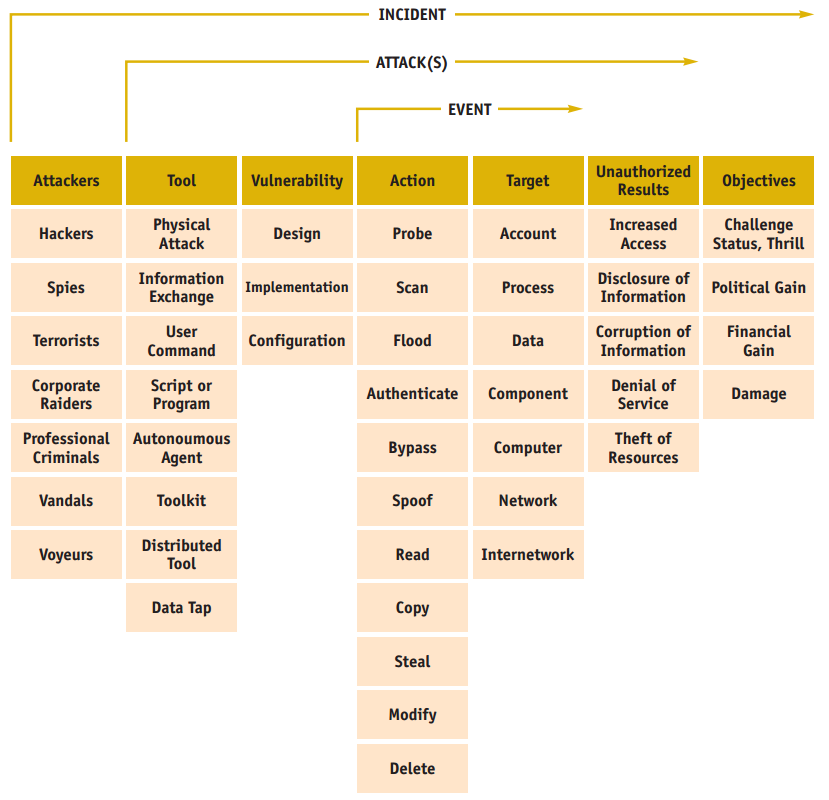
\includegraphics[scale=.4]{images/taxonomia_incidente}
	\caption{Taxonomía de incidentes de seguridad.}
	\label{fig:tax_seg}
\end{figure}


Para que un evento pueda ser considerado así se debe tener conocimiento que una acción, en nuestro caso de estudio debe ser una acción maliciosa, fue o es ejecutada sobre un objetivo, este puede ser cualquier dispositivo conectado a una red dentro de la organización. Para hablar sobre un ataque a una organización se debe de conocer las herramientas usadas, la vulnerabilidad explotada, la acción ejecutada, el objetivo atacado y los resultados no autorizados. Y finalmente para poder considerar que ha ocurrido un incidente de seguridad, la información que se debe conocer es: quién fue la contra-parte, la herramienta usada, la vulnerabilidad, la acción ejecutada, el objetivo atacado, los resultados no autorizados y cuáles fueron los objetivos extraídos del ataque. También en la Figura \ref{fig:tax_seg} viene incluida una taxonomía con ejemplos de las acciones que pueden ser clasificadas dentro de cada etapa de un incidente.\\